
	\section{Плоская монохроматическая волна. Представление монохроматических волн в
		комплексном виде. Сферическая и цилиндрическая волны. Стоячие электромагнитные
		волны. Опыты Винера.}
	(ЛЛ2 \S 46 и дальше)\\
	\subsection*{Плоские волны}
	Стартуем с обычного волнового уравнения:
	\begin{align*}
	\Delta A - \dfrac{1}{c^2} \dfrac{\partial^2}{\partial t^2}A = 0
	\end{align*}
	Где A - это вектор потенциал, так же помним что такое уравнение было полученно при калибровке $\diver A = 0$. Понятно, что для напряженности электрического и магнитного поля верны такие же уравнения. Хотим изучать плоские волны, это значит, что вектор потенциал может зависить только от одной координаты. Для определенности это x. Тогда уравнение выглядит так:
	\begin{align}
	\dfrac{\partial^2}{\partial x^2}\vec{A} - \dfrac{1}{c^2} \dfrac{\partial^2}{\partial t^2}\vec{A} = 0
	\label{7_1eq}
	\end{align}
	Калибровочное условие превращается в $ \dfrac{\partial}{\partial x}A_x = 0$, значит $\dfrac{\partial^2}{\partial t^2}A_x  = 0$. Отсюда логично заключить, что x компонента потенциала либо линейна по времени, либо ее нет. Первое означало бы наличие постоянного электрического поля, что никакого отношения к волнам не имеет. Значит $A_x = 0$. То есть вектор потенциал всегда лежит в плоскости перпендикулярной направлению движения. Для любого, кто читал конспект по матфизу очевидно, что решением уравнения (\ref{7_1eq}) будет любая функция $\vec{A}(t - \dfrac{x}{c})$ понятно что волна еще может лететь влево, но опустим это, там все то же самое. Из этого решения следует, что 
	\begin{align}
	\dfrac{\partial A}{\partial t} = -\dfrac{1}{c} \dfrac{\partial A}{\partial x}
	\label{7_2eq}
	\end{align}
	Пока запомним это. Теперь вычислим E и H, помня, что вектор потенциал зависит только от x
	\begin{align*}
	\vec{H} = - \vec{e}_y \partial_x A_z + \vec{e}_z \partial_x A_y\\
	\vec{E} = -\dfrac{1}{c} \vec{e}_y\dfrac{\partial A_y}{\partial x} -\dfrac{1}{c} \vec{e}_z \dfrac{\partial A_z}{\partial x}\\
	\vec{E}\vec{H} = -\dfrac{1}{c^2} \partial_x A_y \partial_x A_z +\dfrac{1}{c^2} \partial_x A_y \partial_x A_z = 0
	\end{align*}
	Здесь мы воспользовались формулой (\ref{7_2eq}). Теперь мы знаем, что в любой плоской волне электрическое поле перпендикулярно электрическому. И лежат они в одной плоскости, перпендикулярной направлению распространения волны. Кстати, по модулю они равны, что видно из уравнений выше. Так что можно смело написать:
	\begin{align*}
	S = \dfrac{c}{4\pi} [\vec{E} \vec{H}] = \dfrac{c E^2}{4\pi}\vec{n} = \dfrac{cH^2}{4\pi}\vec{n}
	\end{align*}
	Где вектор n единичный в направлении распространения. \\
	Что такое монохроматическая волна? Это когда $\dfrac{1}{c^2} \dfrac{\partial^2}{\partial t^2}\vec{A} =- \dfrac{\omega^2}{c^2} \vec{A}$, фактически фурье компонента. Если подставить это в уравнение (\ref{7_1eq}), то получим обычное уравнение на гармонический осциллятор для координаты. Значит итоговое решение будет:
	\begin{align*}
	\vec{A} = 	Re\{ \vec{A}_0 e^{-i \omega (t - x/c)}\}
	\end{align*}
	Действительную часть мы взяли потому, что поля не бывают комплексными. А вот $A_0$ бывает. Поэтому правильным выбором $A_0$ волну можно сделать любой комбинацией синусов и косинусов которая нужна. Если взять от этой штуки частную производную по времени, что получить поле не сложно:
	\begin{align*}
	\vec{E} = 	Re\{ \vec{E}_0 e^{-i \omega (t - x/c)}\}
	\end{align*}
	Введя вектор $\vec{k} = \dfrac{\omega}{c} \vec{n}$ можно отвязаться от координат и просто написать
	\begin{align*}
	\vec{E} = 	Re\{ \vec{E}_0 e^{i (kr - \omega t)}\}
	\end{align*}
	Обычно взятие действительной части опускают. Так пока мы совершаем линейные операции с полями нам это не важною.  \\
	\subsection*{Сферические и цилиндрические волны}
	Для простоты рассмотрим только монохроматические. Сферические волны это когда зависимость есть только от расстояния до начала координат. Вспоминая как вылгядит оператор лапласа в сферике (например в вики) и быстро решая уравнение получаем (Re опустил):
	\begin{align*}
	A = A_0 \dfrac{e^{i (kr - \omega t)}}{r}
	\end{align*}
	Теперь пишем дифур на цилиндрические волны. \textbf{Здесь r - расстояние до оси}
	\begin{align*}
	&\dfrac{1}{r} \partial_r (r \partial_r f) + k^2 f = 0\\
	& x = r k\\
	&f'' + \dfrac{1}{x} f' + f = 0
	\end{align*} 
	А это уравнение на функцию Бесселя. Конечно есть еще функция Неймана, но нам надо чтобы в нуле значение было конечным, а функция Неймана этого не дает. Итого решениe пропорцианально такой штуке: $J_0(k r) e^{-i\omega t}$ на больших временах можно написать асиптотику: 
	\begin{align*}
	A_0 \dfrac{e^{i (kr - \omega t - \pi/4)}}{\sqrt{r}}
	\end{align*}
	\subsection*{Стоячие волны и опыт Винера}
	Если есть две одинаковые волны $e^{i (kr - \omega t)} \quad e^{i (-kr - \omega t)}$, идущие в разных направлениях (например после отражения), то их можно сложить и получить $2\cos \omega t \cos k r$\\
	Но физически мы можем заметить только квадрат амплитуды. Ну тут видно, что после усреднения по времени мы будем наблюдать серию кучностей на расстоянии по $\lambda/2$ друг от друга. Проблема в их наблюдении это малая длина волны. Вот что придумал Винер.\\
	Берем фоточувствительную пластинку и ставим ее под малым углом к зеркалу. Освещаем зеркало монохроматическим светом на наблюдаем тучности непосредственно
	\begin{figure}[H]
		\centering
		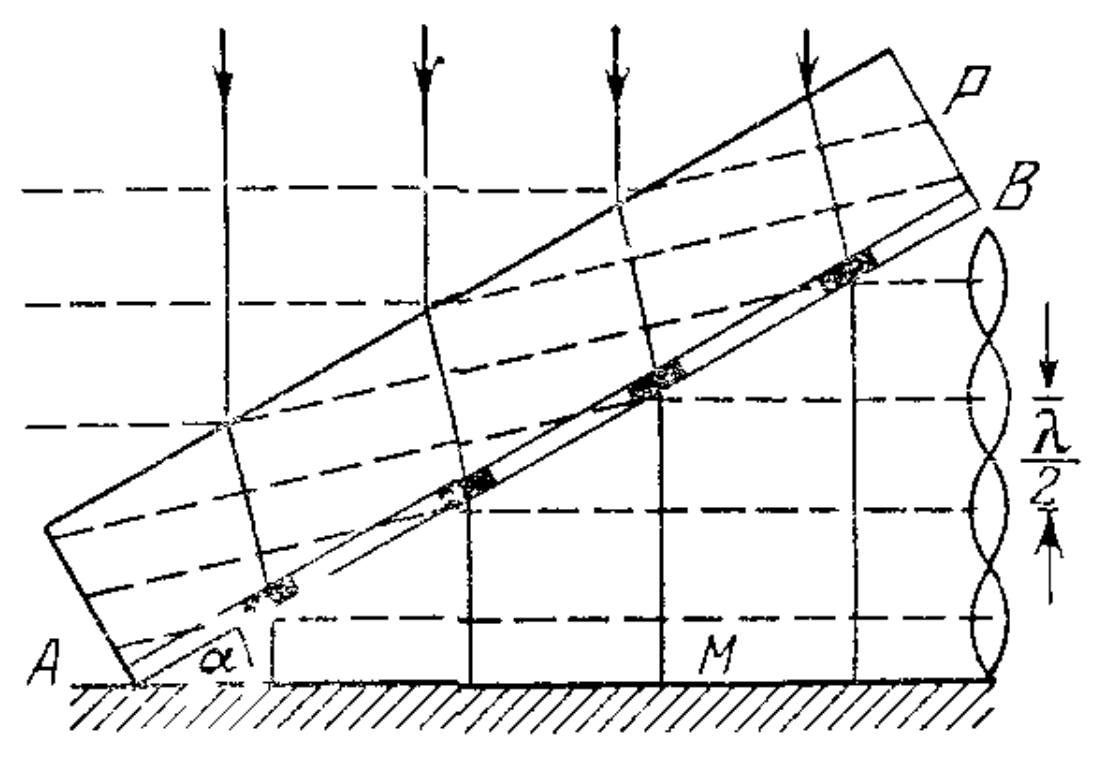
\includegraphics[scale = 0.3]{7_1}
	\end{figure}
	Расстояние между ними по прямой будет $\dfrac{\lambda}{2 \sin \alpha}$, то есть зная синус наклона можно узнать и длину волны.  